\documentclass{beamer}
\usepackage{tikz} % For graphs and graphics
\usetikzlibrary{shapes.geometric, shapes.misc, arrows, positioning}
\def\checkmark{\tikz\fill[scale=0.4](0,.35) -- (.25,0) -- (1,.7) -- (.25,.15) -- cycle;} % Define a checkmark (tick), used in section 2

\graphicspath{ {figures/} }
\setbeamertemplate{page number in head/foot}[totalframenumber]
\usetheme{Marburg}
\newenvironment{system}%
{\left\lbrace\begin{array}{@{}l@{}}}%
{\end{array}\right.}

\beamersetuncovermixins{\opaqueness<1>{25}}{\opaqueness<2->{15}}
\begin{document}
\title{Agent for Bazar Blot}
\author{G. Hovhannisyan,  A. Abrahamyan\\
M. Khachatryan, M. Davtyan}
\date{December 3, 2024}

\AtEndDocument{\begin{frame}
                  \begin{center}
                      Thank You For Attention!\\
                      More Information is available at Our\\
                      \href{https://github.com/aramabrahamyan1703/BeloteAI}{Github Repository}
                  \end{center}
               \end{frame}
                }

\begin{frame}
\titlepage
\end{frame}

\begin{frame}\frametitle{Table of contents}\tableofcontents
\end{frame}


\section{Introduction}
\begin{frame}\frametitle{Introduction}
    \begin{center}
        \textbf{Introduction}
    \end{center}
\end{frame}

\begin{frame}\frametitle{Introduction}
\begin{center}
    \begin{columns}
        \begin{column}{5cm}
        \begin{itemize}
        \item The Origin of the Game
        \item General Rules
        \end{itemize}
        \end{column}
        \begin{column}{2cm}
            \begin{itemize}
                \item Bidding
                \item Playing
            \end{itemize}
        \end{column}
    \end{columns}
    \vspace{15pt}
            \begin{tabular}{|c|c|c|c|}
                \hline
                \textbf{Card} & \textbf{Trump} & \textbf{Regular} & \textbf{No-Trumps}\\
                \hline
                A & 11 & 11 & 19\\
                \hline
                K & 4 & 4 & 4\\
                \hline
                Q & 3 & 3 & 3\\
                \hline
                J & 20 & 2 & 2\\
                \hline
                10 & 10 & 10 & 10\\
                \hline
                9 & 14 & 0 & 0\\
                \hline
                8 & 0 & 0 & 0\\
                \hline
                7 & 0 & 0 & 0\\
                \hline
            \end{tabular}

\end{center}
\end{frame}

\section{Introduction}
\begin{frame}\frametitle{Introduction}
    \begin{center}
        \textbf{Environment Type}
    \end{center}
    \begin{itemize}
        \item Partially Observable
        \item Multi-Agent
        \item Stochastic
        \item Sequential
        \item Static
        \item Discrete
        \item Known
    \end{itemize}
\end{frame}

\section{Auction} 
\begin{frame}\frametitle{Auction}
    \begin{center}
        \begin{itemize}
            \item 6 possible choices for the model
                \begin{itemize}
                    \item Call Hearts
                    \item Call Spades
                    \item Call Clubs
                    \item Call Diamonds
                    \item Call No Trumps
                    \item Pass
                \end{itemize}
            \item Hill-Climbing Algorithm for making the choice
            \item Additional step for determining the call amount (+1, +2, etc.)
        \end{itemize}
    \end{center}
\end{frame}

\begin{frame}\frametitle{Auction}
    Each of the possible calls have their own heuristic value and Hill Climbing algorithm will chose the max out of them.

    \begin{itemize}
    \item $f(Suit)$ = The values associated with the suit if it is chosen as trump + 1/2 $*$ The bid of the Friend of the same suit.
    \item $f(NoTrmps)$ = (The values associated with the suit if it is chosen as trump + 1/2 $*$ The bid of the Friend of the same suit) / 2.
    \item $f(Pass)$ = (Previous Highest Bid) $*$ 4.
    \end{itemize}

    The max will be chosen as the Suit and the value will be the max / 20.

    

\end{frame}

\begin{frame}\frametitle{Auction}
    \begin{center}
    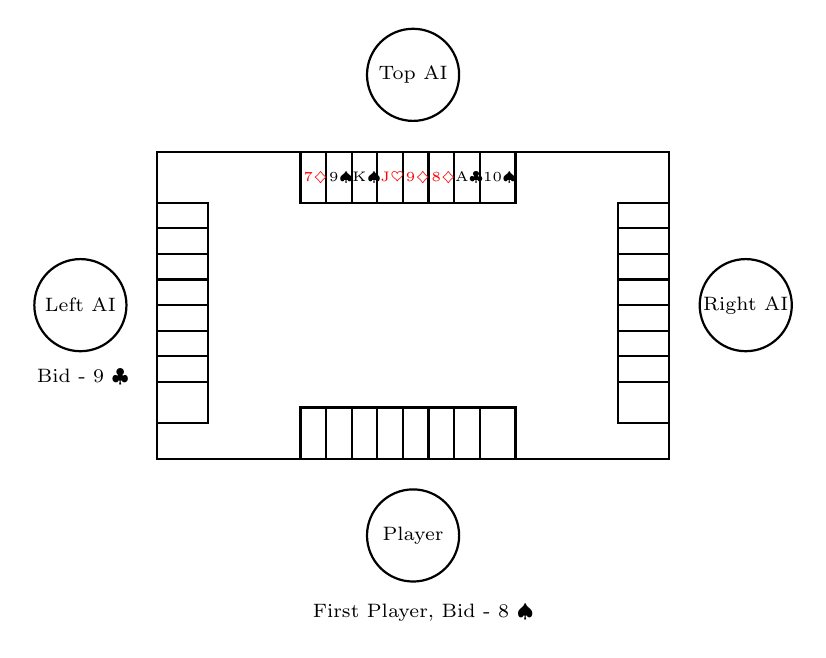
\begin{tikzpicture}[scale=0.65]

        \draw[thick] (0,0) rectangle (10,6);  % Rectangle table dimensions
        
        \foreach \i in {0,1,2,3,4,5,6,7}
            \draw[thick, draw=black, fill=white] (1, 5-\i*0.5) rectangle (0, 5-\i*0.5-0.8);
        \foreach \i in {0,1,2,3,4,5,6,7}
            \draw[thick, draw=black, fill=white] (10, 5-\i*0.5) rectangle (9, 5-\i*0.5-0.8);
        \foreach \i in {0,1,2,3,4,5,6,7}
            \draw[thick, draw=black, fill=white] (2.8 + \i*0.5, 6) rectangle (3.5 + \i*0.5, 5);
        \foreach \i in {0,1,2,3,4,5,6,7}
            \draw[thick, draw=black, fill=white] (2.8 + \i*0.5, 0) rectangle (3.5 + \i*0.5, 1);
        
        \draw[thick] (-1.5, 3) circle(0.9);
        % Right side chair
        \draw[thick] (11.5, 3) circle(0.9);
        % Top side chair
        \draw[thick] (5, 7.5) circle(0.9);
        % Bottom side chair
        \draw[thick] (5, -1.5) circle(0.9);
        
        \node at (-1.5, 3) {\scriptsize Left AI};
        \node at (-1.45, 1.6) {\scriptsize Bid - 9 $\clubsuit$};
        \node at (11.5, 3) {\scriptsize Right AI};
        \node at (5, 7.5) {\scriptsize Top AI};
        \node at (5, -1.5) {\scriptsize Player};
        \node at (5.2, -3) {\scriptsize First Player, Bid - 8 $\spadesuit$};
        
        \node at (3.1, 5.5) {\tiny \textcolor{red}{7$\diamondsuit$}};
        \node at (3.6, 5.5) {\tiny \textcolor{black}{9$\spadesuit$}};
        \node at (4.1, 5.5) {\tiny \textcolor{black}{K$\spadesuit$}};
        \node at (4.6, 5.5) {\tiny \textcolor{red}{J$\heartsuit$}};
        \node at (5.1, 5.5) {\tiny \textcolor{red}{9$\diamondsuit$}};
        \node at (5.6, 5.5) {\tiny \textcolor{red}{8$\diamondsuit$}};
        \node at (6.1, 5.5) {\tiny \textcolor{black}{A$\clubsuit$}};
        \node at (6.7, 5.5) {\tiny \textcolor{black}{10$\spadesuit$}};
        
        \end{tikzpicture}
    \end{center}
\end{frame}

\section{Mini-Max}
\begin{frame}\frametitle{Mini-Max}
    \begin{center}
        \textbf{Mini-Max}
    \end{center}
\end{frame}


\begin{frame}\frametitle{Expectimax}
    Without resorting to cheating we will have $\binom{24}{8}$ nodes in our first depth!\\
    \begin{center}
    \begin{figure}
    \caption{Example of a Game}
    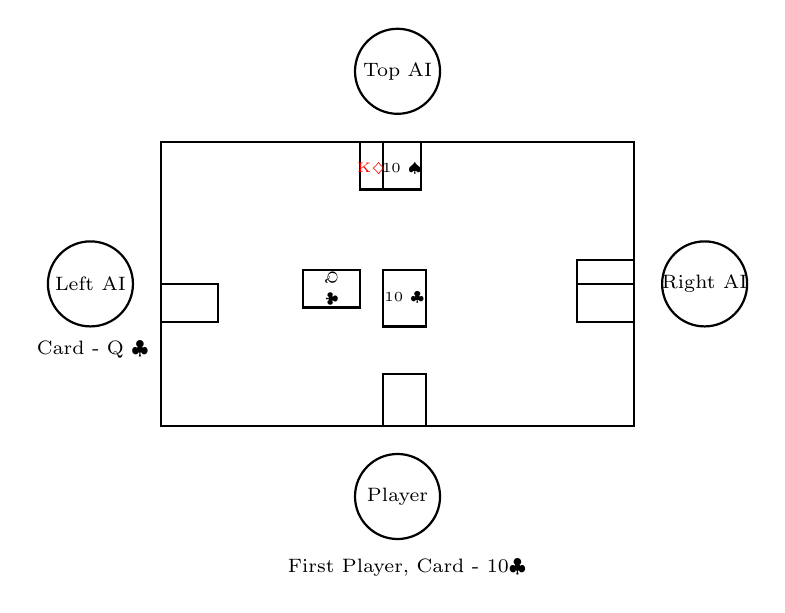
\begin{tikzpicture}[scale=0.6]

        \draw[thick] (0,0) rectangle (10,6);  % Rectangle table dimensions
        
        \draw[thick, draw=black, fill=white] (1.2, 3.5-0.5) rectangle (0, 3.5-0.5-0.8);
        \draw[thick, draw=black, fill=white] (4.2, 3.3) rectangle (3, 2.5);
        \foreach \i in {0,1}
            \draw[thick, draw=black, fill=white] (10, 3.5-\i*0.5) rectangle (8.8, 3.5-\i*0.5-0.8);
        \foreach \i in {0,1}
            \draw[thick, draw=black, fill=white] (5 + \i*0.5, 6) rectangle (4.2 + \i*0.5, 5);
        \draw[thick, draw=black, fill=white] (5.1 + 0.5, 0) rectangle (4.2 + 0.5, 1.1);
        \draw[thick, draw=black, fill=white] (5.1 + 0.5, 3.3) rectangle (4.2 + 0.5, 2.1);
        
        \draw[thick] (-1.5, 3) circle(0.9);
        % Right side chair
        \draw[thick] (11.5, 3) circle(0.9);
        % Top side chair
        \draw[thick] (5, 7.5) circle(0.9);
        % Bottom side chair
        \draw[thick] (5, -1.5) circle(0.9);
        
        \node at (-1.5, 3) {\scriptsize Left AI};
        \node at (-1.45, 1.6) {\scriptsize Card - Q $\clubsuit$};
        \node at (11.5, 3) {\scriptsize Right AI};
        \node at (5, 7.5) {\scriptsize Top AI};
        \node at (5, -1.5) {\scriptsize Player};
        \node at (5.2, -3) {\scriptsize First Player, Card - 10$\clubsuit$};
        
        \node [rotate=270] at (3.6, 2.9) {\tiny \textcolor{black}{Q $\clubsuit$}};
        \node at (5.15, 2.7) { \tiny \textcolor{black}{10 $\clubsuit$}};
        \node at (5.1, 5.45) {\tiny \textcolor{black}{10 $\spadesuit$}};
        \node at (4.45, 5.45) {\tiny \textcolor{red}{K$\diamondsuit$}};
        
        
        \end{tikzpicture}
    \end{figure}
    \end{center}
\end{frame}

\begin{frame}\frametitle{Expectimax}
    \begin{center}
        \begin{figure}
        \caption{Example of Expectimax tree}
	    \includegraphics[width=10cm]{MiniMax_Tree.png}
        \end{figure}
    \end{center}        
\end{frame}


\begin{frame}\frametitle{Cheating Mini-Max}
    \begin{itemize}
        \item Assuming we know everyone's cards what's the approximate number of terminal states?
    \end{itemize}
\end{frame}

\begin{frame}\frametitle{Cheating Mini-Max}
        \begin{itemize}
            \item Assuming we know everyone's cards what's the approximate number of terminal states?
            \item $(8!)^4$
            \item We can't use normal Mini-Max either even with alpha-beta pruning.
        \end{itemize}
\end{frame}

\begin{frame}\frametitle{Depth-Limited Cheating Mini-Max}
    \begin{itemize}
        \item Depth is limited to 12.
        \item Uses alpha-beta pruning.
        \item Heuristic is the current score / 10.
        \item It plays slightly worse than a random bot.
    \end{itemize}
\end{frame}


\section{Simulation Results}
\begin{frame}\frametitle{Simulation Results}
\begin{center}
    \textbf{Simulation Results}
\end{center}
\end{frame}


\begin{frame}\frametitle{Minimax vs Random Without Auction (Three hand version)}
\begin{center}
        \begin{figure}
	    \includegraphics[width=10cm]{ThreeHandMinimax.png}
        \end{figure}
\end{center}
\end{frame}

\begin{frame}\frametitle{Minimax vs Random Without Auction (One hand version)}
\begin{center}
        \begin{figure}
	    \includegraphics[width=10cm]{OneHandMinimax.png}
        \end{figure}
\end{center}
\end{frame}

\begin{frame}\frametitle{Random vs Random Without Auction (Control)}
\begin{center}
        \begin{figure}
	    \includegraphics[width=10cm]{RandomvsRandom.png}
        \end{figure}
\end{center}
\end{frame}

\begin{frame}\frametitle{Combined Plot of the Three Versions}
\begin{center}
        \begin{figure}
	    \includegraphics[width=10cm]{Combined.png}
        \end{figure}
\end{center}
\end{frame}

\begin{frame}\frametitle{Game Results With Auction (Control)}
\begin{center}
        \begin{figure}
	    \includegraphics[width=10cm]{Control.png}
        \end{figure}
\end{center}
\end{frame}

\begin{frame}\frametitle{Game Results With Auction (V1 vs V2)}
\begin{center}
        \begin{figure}
	    \includegraphics[width=10cm]{V1vsV2.png}
        \end{figure}
\end{center}
\end{frame}

\section{Conclusion}
\begin{frame}\frametitle{Conclusion}
    \begin{center}
        \textbf{How to make further improvements}
    \end{center}
    \begin{itemize}
        \item Use Learning Agents 
        \item Monte-Carlo
        \item Further Adjust the Heuristic Values 
        \item Use Other Algorithms Instead of MiniMax
    \end{itemize}
\end{frame}

\end{document}